\selectlanguage{italian}%

\section{Simulazione\label{sim disp}}

Per la simulazione sono state valutate differenti configurazioni degli
ingressi mediante il costrutto \emph{for-loop}.

\lstinputlisting[language=VHDL,caption={Simulazione del componente Display},firstline=71]{esercizio04/codice/display_testbench.vhd}

Di seguito il segnale \emph{values} sar� rappresentato in esadecimale.
In figura \ref{fig:dispsim1} osserviamo come al variare di \emph{values}
segue la commutazione del segnale \emph{cathodes} in modo coerente
al conteggio. Quando infatti il valore di ingresso � pari a \emph{x''0008''},
al primo conteggio i catodi seguono l'ingresso diverso per la prima
cifra. Analogamente per la seconda cifra quando il valore di ingresso
� pari a \emph{x''0010''}.

\begin{figure}[H]
	\centering
	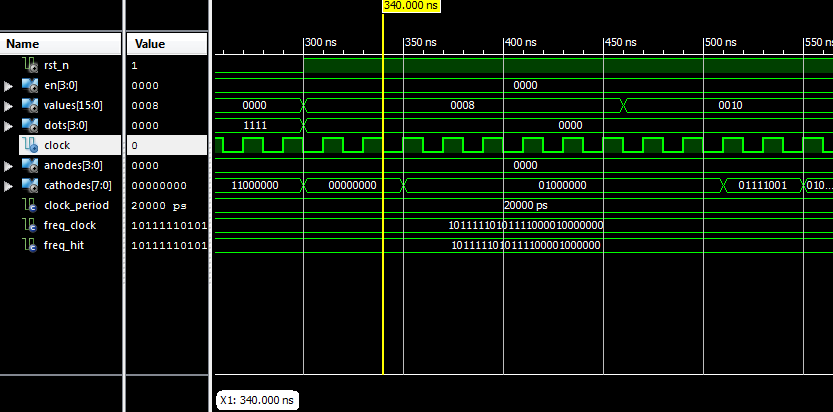
\includegraphics[scale=0.8]{esercizio04/images/Simulazione1.png}
	\caption{Simulazione del display: i catodi seguono correttamente il valore di ingresso per i sette segmenti delle diverse cifre}
	\label{fig:dispsim1}
\end{figure}

In figura \ref{fig:dispsim2} notiamo che, al variare di \emph{en}
e \emph{dots}, segue la commutazione di \emph{anodes} e \emph{cathodes},
coerentemente al valore di conteggio. Quando, infatti, i segnali di
abilitazione e dei punti sono pari a x\emph{''0100''}, al conteggio
associato alla terza cifra seguono nella commutazione anche il relativo
anodo e il catodo che rappresenta il punto.

\begin{figure}[H]
	\centering
	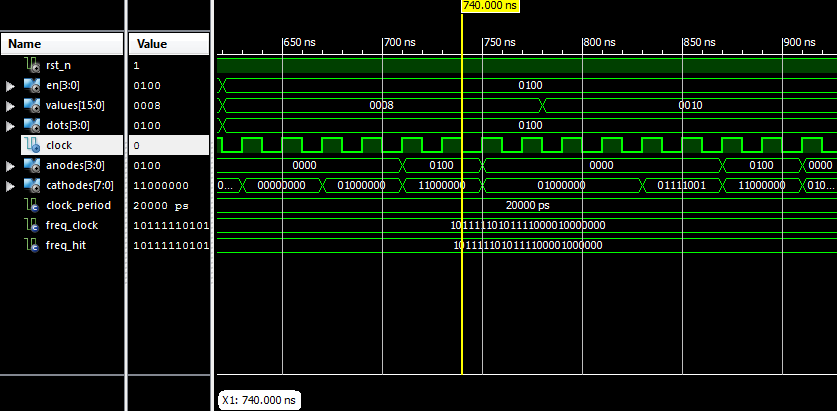
\includegraphics[scale=0.8]{esercizio04/images/Simulazione2.png}
	\caption{Simulazione del display: gli anodi seguono correttamente i valori di abilitazione; il catodo del punto segue correttamente i valori dei punti}
	\label{fig:dispsim2}
\end{figure}

Con \emph{rst\_n} pari a 0, ovvero il segnale di reset attivo, il
conteggo si blocca alla prima cifra. Osserviamo in figura \ref{fig:dispsim3}
che le uscite segnano identicamente i valori relativi alla prima cifra,
indipendentemente dalla variazione degli altri ingressi. Esse infatti
non sono sensibili alle variazioni di \emph{en} e \emph{dots} sulla
terza cifra (\emph{``0100''}), ma notiamo una commutazione al variare
di \emph{values} sulla prima cifra (\emph{x''0008''}).

\begin{figure}[H]
	\centering
	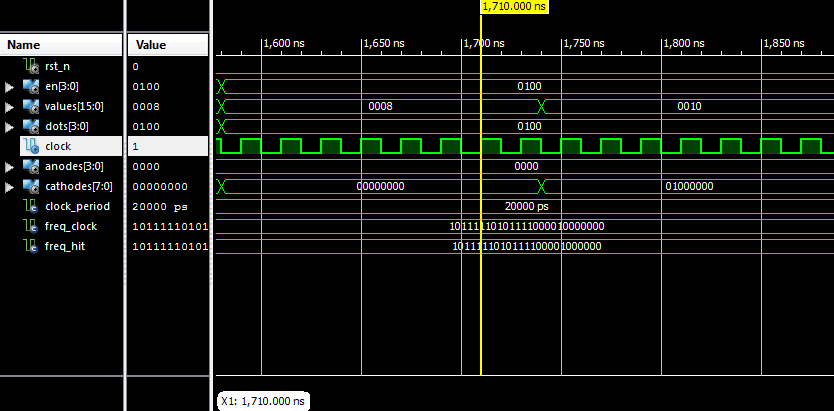
\includegraphics[scale=0.8]{esercizio04/images/Simulazione3.png}
	\caption{Simulazione del display: il reset basso blocca il conteggio alla prima cifra}
	\label{fig:dispsim3}
\end{figure}\selectlanguage{italian}%

